%!TEX root = master.tex
\section{Astronomical imaging: \\ Telescopes and Doppler imaging}
Astronomers need telescopes to collect photons from planets, stars and distant galaxies, track the objects on the sky and to create the image of a region on the sky. They strive to limit the FOV "Field of view" which can be done with large primary mirrors in the telescopes. Some examples of large telescopes:

\begin{itemize}
	\item ELT, 39m 
	\item LBT 2 $\times$ 11.8m
	\item Keck I \& II 2 $\times$ 10m 
\end{itemize}

All newer telescopes are tracking the objects on the sky with the Alt-Azimuth mount. Other mount are: 
\begin{itemize}
	\item German mount
	\item Fork mount
	\item English mount
\end{itemize}

	\subsection{Imaging: the points spread function}
	An image of a Point Spread Function, "PSF" created by a telescope is not a point due to diffraction. The intensity distribution in the focal plane produced by a point source located at infinity is the PSF. The ideal PSF for a circular mirror takes the shape of the Bessel function.

	\textcolor{red}{Image bessel} 

	The resolution or the width of the peak is defined by the ratio of wavelength to the diameter of the telescope. So if we increase the diameter of the mirror it reduces the width of the peak. Using the sampling Theorem: 

		\begin{wbox}{Whittaker-Nyquist-Kotelnikov-Shannon sampling theorem}
			The sampling frequency must be at least twice the highest frequency of the signal.
		\end{wbox}	 

	 (Which has many names due to many worked with the problem in many different fields) gives us the minimum spacing between two Gaussians with a given width so we can tell them apart.

		 \begin{equation}
		 	\text{PSF} \propto \frac{-x^2} {e^{2\sigma^2}} = \frac{1} {2} \Rightarrow x  \equiv \delta = \sqrt{2 \text{ln}2\sigma} \text{ and the separation } = 2\delta= 2  \sqrt{2 \text{ln}2\sigma} \approx 2.355 \cdot \sigma 
		 \end{equation}

	The magical number in astronomy is therefore: 2.355 for sampling. This is important for making sure that we use a sensor that doesn't have to large pixels or smaller than necessary. 

	\subsection{Resolution limit}
	Details that are smaller than the diffraction image of the telescope are smeared out, so after data reduction are anything smaller than $\frac{\lambda} {D} $ an artifact. So, is it possible to do better than the limit set by : $\frac{\lambda} {D} $, can we resolve features of distant objects smaller than the diffraction limit? YES!

		\begin{itemize}
		  	\item Interferometry 
		  	\item Doppler imaging
		  \end{itemize}  
	
	Using data from two telescopes we can try to overlap the images with an adjustable optical path way such the difference in optical path is zero (exact to the fraction of the wavelength). This result in the characteristic interference pattern: fringes which has amplitude and phase that we can analyze and use. By doing this its possible to create larger telescopes (but its not perfect). The fourier harmonics of the data gives us 6 points when using 4 telescopes. When the earth rotates it changes the projected baseline so it must be corrected during the night. 

	Using this technique made it possible to see the changes of the star Betelgeuse intensity change during 2019 in greater detail. With interferometry is the angular resolution limited by the ratio $\frac{\lambda} {B} $ where B is the the distance between the telescopes projected on the line of sight, see figure: \textcolor{red}{fix ref to pic} 	 

		\begin{figure}[ht!]
		 \centering
		 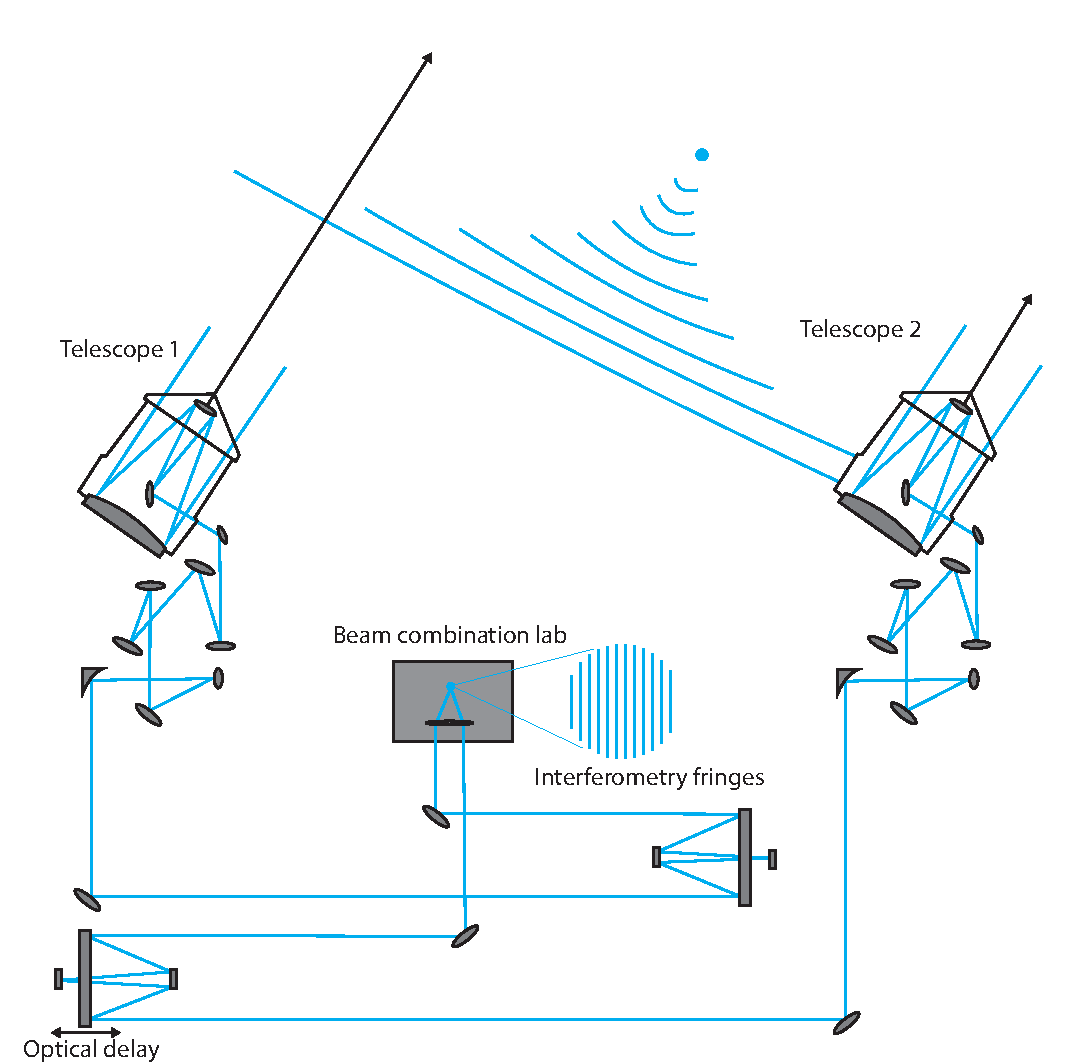
\includegraphics[width=80mm]{figures/telescopes.pdf}
		 \caption{Example of caption}
		 \label{fig:example}
		 \end{figure}
	  
	 Radio interferometers are easier since the wavelength is longer making it cheaper to build and use. Here we can digitize the signal and transmit it with fiber cables instead of highly accurate mirrors and trolleys. The correlation between the telescopes can be done in supercomputers so its just to move the telescopes around and keep track of the position of them. This means that the array can be made more compact, not loosing a lot of flux. 

	 \subsection{Doppler imaging}
	 During the 1900 century astronomers discovered a class of stars that we call "Peculiar". They have a chemical compositions of a lot of rare-earth metals which is unusual. The spectra of the star also showed a periodic variability. After systematic observations of these changes, it became clear that it was not only the strength of the spectral lines that changed but also the shape of them. It later became clear that these stars are fast rotating and have chemical spots on the surface. 

	 These spots of chemicals gives a Doppler effect when rotating around the star, blue shift when the cloud moves towards the observer, the spectrum then appears to be broaden. Setting up the \textbf{forward problem} some assumptions were made: 

		\begin{itemize}
			\item Each observed spectrum is taken during the time that is much shorter than the rotation period
		   	\item The surface structure doesn't change during the observing run
		   	\item The rotational broadening is resolved by our instrument: spectrometer. 
		   	\item The star rotates as a solid body
		\end{itemize}  

	Continuing with setting up the formulation of the forward problem:
		
		\begin{itemize}
			\item The telescope and spectrometer measure the flux coming from the star at a given wavelength and phase: 
			\begin{equation}
			 	F(\lambda, \phi) = \oint I(\lambda + \Delta^{\text{Dop}}_m,m)\cos \theta_m d \sigma_m
			 \end{equation} 
			 \item Intensity I can be computed from a physical model of the stellar atmosphere locally parameterized by chemical composition
			 \item Changes in composition along the stellar surface change the emerging I
		\end{itemize}

	The algorithm: 

		\begin{itemize}
			\item For a given distribution of abundances, compute intensities for each surface element at each phase (non-linear)
			\item Integrate the intensities over the disk to obtain fluxes while taking into account Doppler shifts for all phases(convolution)
			\item Compare the synthetic spectra with observations
			\item Adjust the map(s) of abundance 
		\end{itemize}

	This is an ill-posed problem and belongs to the class of integral equations: \textbf{Fredholm equations}. The properties of the DI kernel makes the problem ill-posed. Take as an example, if we would add a chess pattern to the surface with small/unresolved squares, it would not change the observed spectra? \textcolor{red}{meaning?}

	\subsection{Remote sensing problems}
	Doppler imaging is an example of remote sensing problems. These types of problems arrise when it is impossible or impractical to reach the actual target and measure it properly. What we do instead is to measure other properties that are related to what we want to measure with linear or non-linear transformations. Many of these problems are ill-posed (interferometric image reconstruction is an example). The solution to this is to introduce regularization.

	Solving an inverse problem we need: 

	\begin{itemize}
	    	\item Assume an initial guess for the abundance map
	    	\item Compute the local line profiles
	    	\item integrate over the disk for each of the rotations phases, taking Doppler shifts into account
	    	\item Find the correlations to local abundance that minimize the functional:
		    	\begin{equation}
		    		\sum_{\lambda, \phi}^{}\begin{bmatrix} F^{\text{obs}}_\lambda(Z,\phi - F^{\text{calc}}_\lambda(Z,\phi)^2 \end{bmatrix} + \Lambda \cdot \text{R}(Z) = \text{min}	  
		    	\end{equation} 
		    \item Loop from the second point until convergence is reached. Example of \textbf{R} is Tikhonov regularization:
			    \begin{equation}
			    	\text{\textbf{R}}(Z) ) \sum_{\text{surface}}^{}(\overline{\nabla} Z)^2 
			    \end{equation}
	    \end{itemize}

	\subsection{Extension of Doppler imaging}
	Doppler imaging is also used for monitoring active regions on solar-types starts (solar spots) where temperature variation influences line intensity differences. Can also be used for binary systems which is eclipsing (eclipsing binaries) were the geometry becomes more complex due to the eclipses. Can also be used for medical imaging such as computer aided tomography. 

	\subsection{Conclusion}
	The inverse problems are used to infer information about an object that is not possible to measure directly. The solution in these cases are not often unique. For such cases we replace the problem with a regularized inverse problem. There exist various forms of regularization. 
	        











	 
